The main characteristic of LM rules is that they are constrained by the first
argument\footnote{In the implementation, the first argument of each fact is not
stored.}. Rule derivation uses only facts from the same node, therefore there is
no need to synchronize with other nodes to derive rules. However, when nodes
derive non-local facts (owned by other nodes), then the implementation must
synchronize and \emph{send} the facts to the target node. From the point of view
of the receiving node, these are called \emph{incoming facts}. Note that this is related
to the parallel aspects of the virtual machine and more details are given in the
next chapter.

During the lifetime of a program, each node goes through different states as
specified by the state machine. Figure~\ref{fig:local:node_states} presents the
state machine with the valid state transitions.  In the \textbf{running} state,
the node is deriving rules. In the \textbf{inactive} state, the node has no new
facts to be considered and all candidate rules have been tried. In the
\textbf{active} state, the node has new facts to be considered but is waiting to
be executed by a thread. Finally, in the \textbf{stealing} state, the node is
currently being stolen by some thread.

\begin{figure}[ht]
   \centering
   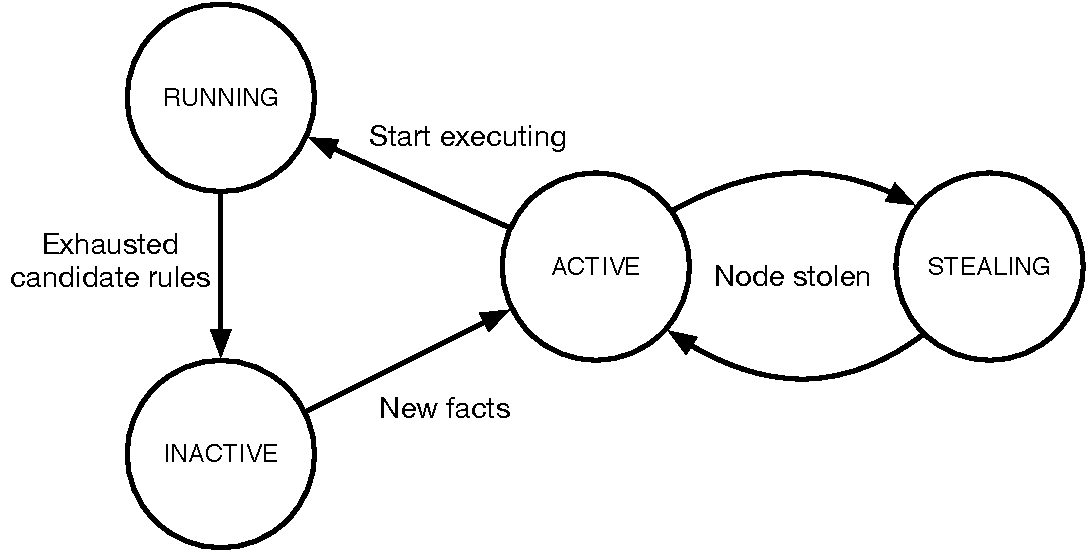
\includegraphics[width=0.55\textwidth]{figures/local/node_state.pdf}
   \caption{The node state machine as represented by the state variable.}
   \label{fig:local:node_states}
\end{figure}

As shown in Fig.~\ref{fig:local:node_overview}, each node contains the
following attributes:

\begin{itemize}
   \item \emph{State}: the node state flag.
   \item \emph{Main Lock}: a lock that protects the node attributes enumerated
      in this list except for \emph{Linear DB}, \emph{Persistent DB}, and
      \emph{Rule Engine}.
   \item \emph{DB Lock}: a lock that protects \emph{Linear DB},
      \emph{Persistent DB} and \emph{Rule Engine}. The lock is held when the node is deriving rules or
      when incoming facts from other nodes need to be added to the database data
      structures.
   \item \emph{Rule Engine}: a data structure that detects which rules are
      candidates and should be derived. The data structure is fully explained
      in Section~\ref{section:local:rule_engine}.
   \item \emph{Owner}: a pointer to the thread responsible for executing this
      node.
   \item \emph{Fact Buffer}: a data structure that holds incoming facts that
      could not be added to the database data structures since the node is
      currently deriving rules.
   \item \emph{Linear DB}: the database of linear facts as an array of data
      structures for storing linear facts for each linear predicate.
   \item \emph{Persistent DB}: the database of persistent facts.
\end{itemize}

\begin{figure*}[t]
\centering
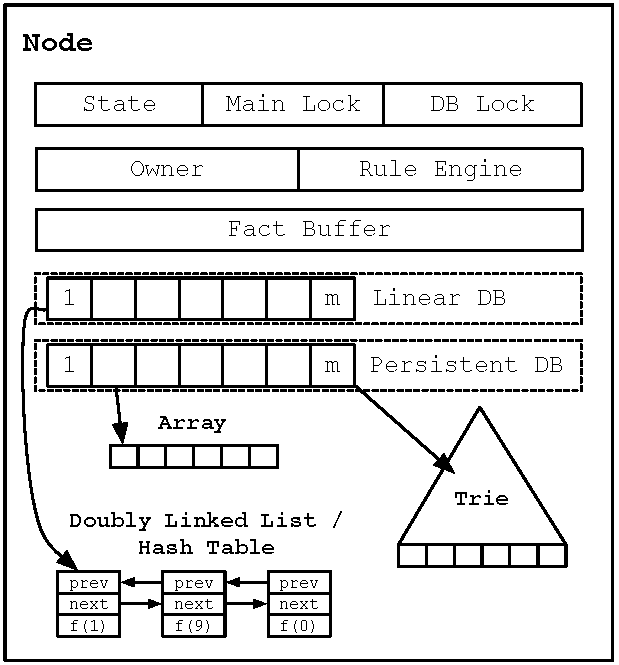
\includegraphics[width=0.5\textwidth]{figures/local/node.pdf}
\caption{Layout of the node data structure.}
\label{fig:local:node_overview}
\end{figure*}

The database of facts must be implemented efficiently because during matching of
rules we need to restrict the facts using \emph{join constraints}, which fix
arguments of predicates to instantiated values. A database fact is made up of 2
pointers (\code{prev} and \code{next}) and a variable number of arguments.  Each
fact argument is large enough to contain a value of any of the available LM
types. Each predicate of the program is stored in a different data structure in
order to make it easier to lookup facts by predicate. Predicate facts are stored
in one of the four data structures:

\begin{itemize}

\item \emph{Trie Data Structures} are used to store persistent facts. Tries are
   trees where facts are indexed by common prefix arguments. The \code{prev}
   and \code{next} pointers are used to store all the facts stored in the trie.

\item \emph{Array Data Structures} are used to store persistent facts that are
   used in the LHS of rules without matching (no join constraints) and exist
   only as initial facts. Facts stored in this data structure do not have the
   \code{prev} and \code{next} pointers because they are already chained by
   being part of a contiguous memory area. The compiler performs static analysis
   of the program's rule in order to choose between trie and array data
   structures for a particular predicate.

\item \emph{Doubly Linked List Data Structures} are used to store linear facts.
   We use a double linked list because it is a very efficient way to add and
   remove facts. The \code{prev} and \code{next} pointers are used to chain
   the facts of the linked list.

\item \emph{Hash Table Data Structures} are used to improve lookup when linked
   lists are too long and when we need to do search filtered by a fixed
   argument. The virtual machine decides which arguments are best to be indexed
   (see Section~\ref{sec:implementation:indexing}) and then uses a hash table
   indexed by the appropriate argument. If we need to go through all the facts,
   we just iterate through all the facts in the table. For collisions, we use
   the doubly linked list data structure mentioned above.

\end{itemize}

Figure~\ref{fig:implementation:hash_table} shows an example for a hash table
data structure for a \code{p(int, int)} predicate with 4 linear facts indexed by
the second argument. Note that for each bucket, facts are stored in a doubly
linked list using the \code{prev} and \code{next} pointers of each fact.

\begin{figure}[ht]
   \centering
   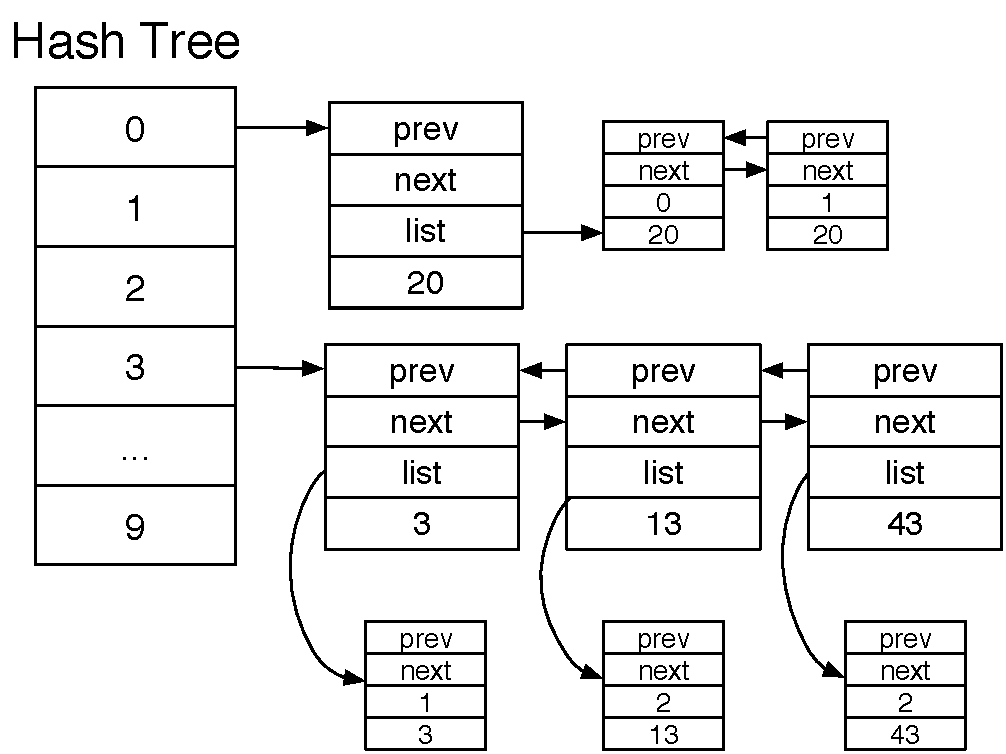
\includegraphics[width=0.6\textwidth]{figures/implementation/hash_table.pdf}

   \caption{Hash table and doubly linked data structures for a \texttt{p(int,
   int)} predicate containing the following facts: \code{p(0, 20)}, \code{p(1,
   3)}, \code{p(2, 13)}, and \code{p(2, 43)}. Facts are indexed by computing
   $arg_2\mod{}10$ where $arg_2$ is the second argument of the fact.}

   \label{fig:implementation:hash_table}
\end{figure}

%%%%%%%%%%%%%%%%%%%%%%%%%%%%%%%%%%%%%%%%%%%%%%%%%%%%%%%%%%%%%%%%%%%%%%

\subsection{Indexing}\label{sec:implementation:indexing}

To improve fact lookup, the VM employs a fully dynamic mechanism to
decide which argument may be optimal to index.  The algorithm is
executed along with normal computation and empirically tries to
assess the argument of each predicate that more equally spreads the
database across the values of the argument. 

The indexing algorithm is performed in three main steps. First, it gathers
lookup statistics by keeping a counter for each predicate's argument. Every time
a fact search is performed where arguments are fixed to a value, the counter of
such arguments is incremented. This phase is performed during rule execution for
100 nodes or 1\% of the nodes of the graph, if the graph has more than 100000
nodes.

The second step of the algorithm selects the candidate arguments of each
predicate. If a predicate was not searched with any fixed arguments, then it
will be not indexed as there are no candidates. If only one argument was fixed,
then such argument is the only available candidate argument and thus immediately
becomes the indexing argument. Otherwise, the top 2 arguments are selected for
the third phase, where \emph{entropy statistics} are collected dynamically.

During the third phase, each candidate argument has an entropy score. Before a
node is executed, the facts of the target predicate are used in the following
formula applied for the two arguments:

\[
Entropy(F, A) = - \sum_{v \in values(F, A)} \frac{count(F, A = v)}{total(F)} \log_2 \frac{count(F, A = v)}{total(F)}
\]

\noindent where $A$ is the target argument, $F$ is the set of linear facts for
the target predicate, $values(F, A)$ is set of values of the argument $A$,
$count(F, A = v)$ counts the number of linear facts where argument $A$ is equal
to $v$ and $total(F)$ counts the number of linear facts in $F$.  The entropy
value is a good metric because it tells us how much information is needed to
describe an argument. If more information is needed, then that must be the best
argument to index.

For each arguments, the $Entropy(A, F)$ value is then multiplied by the number
of times it has been used for lookup. The argument with the best score is
selected and then a global variable called \texttt{indexing\_epoch} is updated
to \textbf{completed}. In order to convert the node's linked lists into hash
tables, each node also has a local variable called \texttt{indexing\_epoch} that
is compared to the global variable in order to rebuild the database according to
the new indexing information.

The VM also dynamically resizes the hash table if necessary. When the hash table
becomes too dense, it is doubled in size. When it becomes too sparse, it is
reduced in half or simply transformed back into a doubly linked list. This is
done once in a while, before a node executes.

We have seen very good results with this scheme. The overhead of dynamic
indexing is negligible since programs run almost as fast as if the indices have
been added from the start. However, the programmer can still index predicates
statically, if needed, using the directive \code{index pred/arg}, where
\code{pred} is the argument name and \code{arg} is the argument number to index.
